\section{Gravity waves}
\label{sec:theory:gw}

When an air parcel is forced to rise over a mountain, it experiences a restoring buoyancy force which can create waves that propagate away from the mountain.  These are known as gravity waves, mountain waves, or lee waves.  

Gravity waves play an important role in mesoscale weather.  The waves can trigger convection by propagating through areas of weak stability, they cause clear-air turbulence that affects aircraft \autocite{ray1986}, and can produce very strong downslope winds on the lee slope of the mountain \autocite{holton2003}.

In this section, we briefly present the theory of linear waves and demonstrate their effect on wind and temperature.  In section~\ref{sec:gw}, we relate this theory to the results of a two dimensional experiment in which gravity waves are induced by flow over a wave-shaped mountain range.

Two dimensional waves in the $x-z$ plane are characterised by their frequency, $\omega$, amplitude $\amplitude$, and their horizontal and vertical wavenumbers, $k$ and $m$.  In flow over a mountain, the horizontal wavenumber is often related to the spacing between mountain ridges.  By starting with the Boussinesq approximation of the Navier-Stokes equations we can derive the dispersion relation \autocite{lynch-cassano2006}
\begin{align}
	\left( \frac{\partial}{\partial t} + \overline{u} \frac{\partial}{\partial x} \right)^2
	\left( \frac{\partial^2 w'}{\partial x^2} + \frac{\partial^2 w'}{\partial z^2} \right) +
	N^2 \frac{\partial^2 w'}{\partial x^2} = 0
%
	\intertext{where $\overline{u}$ is the mean horizontal wind and $w'$ is the vertical velocity anomaly.  This can be solved by assuming a wave-like solution}
%
	w' = \amplitude \cos \left( kx + mz - \omega t \right) \label{eqn:theory:gw:w-prime}
	\intertext{thus giving the dispersion relation}
	\left( \omega - \overline{u}k \right)^2 
	\left( k^2 + m^2 \right) -
	N^2 k^2 = 0 \label{eqn:theory:gw:dispersion}
\end{align}

The potential temperature anomaly $\theta'$ is a function of background stability $\partial \overline{\theta}/\partial z$ and is \ang{90} out of phase with $w'$, given by \autocite{lynch-cassano2006} \TODO{it'd be nice to derive this from Boussinesq equations but I've struggled to do it myself}
\begin{align}
	\theta' &= \frac{\amplitude}{\omega} \frac{\diff{\overline{\theta}}}{\diff{z}} \sin \phase \label{eqn:theory:gw:theta-prime}
%
	\intertext{where the phase $\phase$ is}
%
	\phase &= kx + mz - \omega t \label{eqn:theory:gw:phase}
\end{align}

\begin{figure}
	\centering
	\documentclass[tikz]{standalone}
\usepackage{bm}
\usetikzlibrary{arrows}
\newcommand{\vect}{\bm}
\newcommand{\del}{\nabla}

\newcommand{\trans}[1]{{#1^\star}}
\newcommand{\surface}{h}
\newcommand{\shellcmd}[1]{\texttt{#1}}
\newcommand{\diffusioncoeff}{\mathcal{D}}
\newcommand{\exner}{\Pi}
\newcommand{\courant}{\mathrm{Co}}

\begin{document}
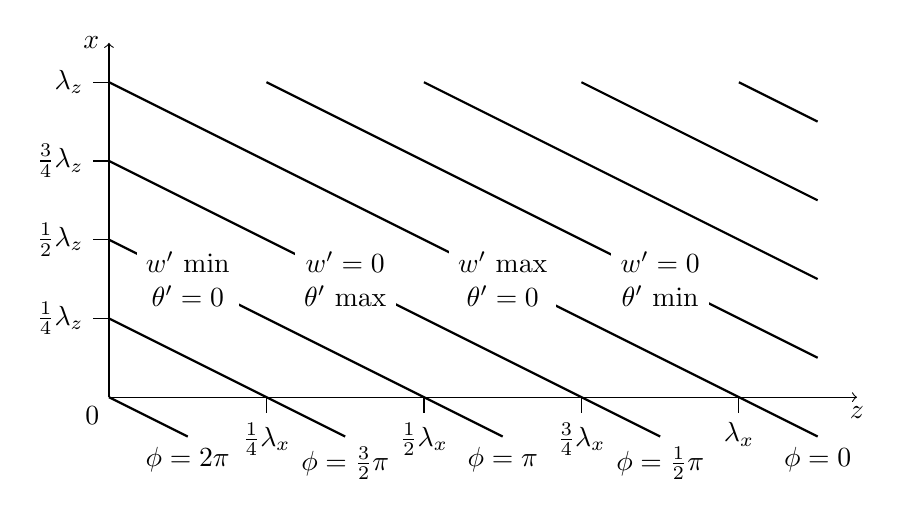
\begin{tikzpicture}[
  cpnt/.style={fill=gray},
  arr/.style={thick, ->},
]
\draw [->] (0,0) -- (0,4.5) node [at end, anchor=east] {$x$} node [at start, anchor=north east] {$0$};
\draw [->] (0,0) -- (9.5,0) node [at end, anchor=north] {$z$};

\draw [thick] (0,0) -- (1,-0.5) node [at end, anchor=north] {$\phi = 2 \pi$};
\draw [thick] (0,1) -- (3,-0.5) node [at end, anchor=north] {$\phi = \frac{3}{2} \pi$};
\draw [thick] (0,2) -- (5,-0.5) node [at end, anchor=north] {$\phi = \pi$};
\draw [thick] (0,3) -- (7,-0.5) node [at end, anchor=north] {$\phi = \frac{1}{2} \pi$};
\draw [thick] (0,4) -- (9,-0.5) node [at end, anchor=north] {$\phi = 0$};
\draw [thick] (2,4) -- (9,0.5);
\draw [thick] (4,4) -- (9,1.5);
\draw [thick] (6,4) -- (9,2.5);
\draw [thick] (8,4) -- (9,3.5);

\node [fill=white, align=center] at (1,1.5) {$w'$ min\\$\theta' = 0$};
\node [fill=white, align=center] at (3,1.5) {$w' = 0$\\$\theta'$ max};
\node [fill=white, align=center] at (5,1.5) {$w'$ max\\$\theta' = 0$};
\node [fill=white, align=center] at (7,1.5) {$w' = 0$\\$\theta'$ min};

\draw (0,1) -- (-0.2,1) node [at end, anchor=east] {$\frac{1}{4} \lambda_z$};
\draw (0,2) -- (-0.2,2) node [at end, anchor=east] {$\frac{1}{2} \lambda_z$};
\draw (0,3) -- (-0.2,3) node [at end, anchor=east] {$\frac{3}{4} \lambda_z$};
\draw (0,4) -- (-0.2,4) node [at end, anchor=east] {$\lambda_z$};

\draw (2,0) -- (2,-0.2) node [at end, anchor=north] {$\frac{1}{4} \lambda_x$};
\draw (4,0) -- (4,-0.2) node [at end, anchor=north] {$\frac{1}{2} \lambda_x$};
\draw (6,0) -- (6,-0.2) node [at end, anchor=north] {$\frac{3}{4} \lambda_x$};
\draw (8,0) -- (8,-0.2) node [at end, anchor=north] {$\lambda_x$};

\end{tikzpicture}
\end{document}

	\caption{Phase relationship between vertical velocity anomalies $w'$ and potential temperature anomalies $\theta'$.  Adapted from \textcite{lynch-cassano2006}.}
	\label{fig:theory:gw:phases}
\end{figure}

Using equations~\ref{eqn:theory:gw:w-prime}, \ref{eqn:theory:gw:theta-prime} and \ref{eqn:theory:gw:phase} we can plot the phase relationships between $w'$ and $\theta'$, shown in figure~\ref{fig:theory:gw:phases}.

Next, we impose a lower boundary condition to simulate flow over an infinite, wave-shaped terrain and find that two types of stationary wave exist.  Consider a surface, the height of which is defined by $h(x)$, such that
\begin{align}
	h(x) &= h_0 \cos \left( kx \right)
%
	\intertext{The flow at any point at the surface must be parallel to that surface (that is, a no normal flow boundary condition)}
%
	w(x,0) &= \frac{\diff{h}}{\diff{t}} \\
	  &= \overline{u} \frac{\partial h}{\partial x} \\
	  &= - \overline{u} k h_0 \sin \left( kx \right) \label{eqn:theory:gw:boundary-cond}
%
	\intertext{Assuming a stationary wave in the form $w'(x, z) = - \overline{u} k h_0 \sin \left( kx + mz \right)$, and noting that $\partial / \partial t = 0$ and $\omega = 0$, we find that the dispersion relation given by equation~\ref{eqn:theory:gw:dispersion} has the solution \autocite{lynch-cassano2006}}
%
	m &= \sqrt{\frac{N^2}{\overline{u}^2} - k^2} \label{eqn:theory:gw:m-dispersion}
\end{align}
which also satisfies the boundary condition given by equation~\ref{eqn:theory:gw:boundary-cond}.  The solution is presented in figure~\ref{fig:theory:gw:propagating} which shows the vertically propagating wave.

We see from equation~\ref{eqn:theory:gw:m-dispersion} that, for $m$ to have a real solution, $|\overline{u}k| < N$.  This constraint cannot be satisfied when the wind is too strong, stability is too weak, or the spacing of mountain ridges is too narrow (that is, $k$ is too large).  In this case, the dispersion relation is instead satisfied by the solution \autocite{lynch-cassano2006}
\begin{align}
	w' &= - \overline{u} k h_0 e^{-mz} \sin \left( kx \right)
\end{align}
As shown in figure~\ref{fig:theory:gw:evanescent}, in this solution, waves decay with height and there is no vertical propagation.  These are often called evanescent waves.

\begin{figure}
	\centering
	\captionsetup[subfigure]{position=b}
	\centering
	\subcaptionbox{Vertically propagating gravity wave \label{fig:theory:gw:propagating}}[0.48\textwidth]{\input{gravityWaves-propagating-plot}}
	\hfill
	\subcaptionbox{Evanescent wave showing rapid decay decay in height and no vertical propagation \label{fig:theory:gw:evanescent}}[0.48\textwidth]{\input{gravityWaves-evanescent-plot}}
%
	\caption{Example vertical cross sections of streamlines for stationary gravity waves over infinite sinusoidal terrain.  Thick dashed lines denote lines of constant phase.  Adapted from \textcite{lynch-cassano2006}.}
	\label{fig:theory:gw:stationary-waves}
\end{figure}

